\subsection{Penalty-based formalism}

\begin{algorithm}
	\protect\caption{\label{alg4}MATLAB Penalty Solver.}
	\begin{algorithmic}[1]
	\Function{Penalty}{A, B, C, D, E, F, rho, tol}

		\State $BA~=~B-A;~CA~=~C-A;~ED~=~E-D;~FD~=~F-D;$

		\State $hf~=~{[}2{*}BA{*}BA',~2{*}CA{*}BA',-2{*}ED{*}BA',-2{*}FD{*}BA';$

		\State $2{*}BA{*}CA',~2{*}CA{*}CA',-2{*}ED{*}CA',-2{*}FD{*}CA';$

		\State $2{*}BA{*}ED',-2{*}CA{*}ED',~2{*}ED{*}ED',~2{*}FD{*}ED';$

		\State $2{*}BA{*}FD',-2{*}CA{*}FD',~2{*}ED{*}FD',~2{*}FD{*}FD'{]};$

		\State $x~=~{[}0.33;~0.33;~0.33;~0.33{]};$

		\For{i=1:99}

			\State $X~=~A+BA{*}x(1)~+~CA{*}x(2);$

			\State $Y~=~D+ED{*}x(3)~+~FD{*}x(4);$

			\State $gf~=~{[}2{*}(X-Y){*}BA';~2{*}(X-Y){*}CA';~-2{*}(X-Y){*}ED';~-2{*}(X-Y){*}FD'{]};$

			\State $h~=~{[}-x(1);~-x(2);~x(1)+x(2)-1;~-x(3);~-x(4);~x(3)+x(4)-1{]};$

			\State $dh~=~{[}-1,~0,~1,~0,~0,~0;~0,~-1,~1,~0,~0,~0;$

			\State $0,~0,~0,~-1,~0,~1;~0,~0,~0,~0,~-1,~1{]};$

			\State $mask~=~h'~$>$=~0;$

			\State $dmax~=~dh.{*}~{[}mask;~mask;~mask;~mask{]};$

			\State $gra~=~gf~+~rho~{*}~dmax~{*}~max(0,h(:));$

			\State $hes~=~hf~+~rho{*}dmax{*}dmax'~+~eye(4,4)/rho^2;$

			\State $dx~=~hes\textbackslash{}gra;$

			\State $DX~=~BA{*}dx(1)~+~CA{*}dx(2);$

			\State $DY~=~ED{*}dx(3)~+~FD{*}dx(4);$

			\State $error~=~sqrt(DX{*}DX'+DY{*}DY');$

			\If{error~$<$~tol}
				\State $BREAK;$
			\EndIf

			\State $x~=~x~-~dx;$

		\EndFor

	\EndFunction
	\end{algorithmic}

\end{algorithm}

penalty vectorization

\begin{figure}[!h]
\centering
\includegraphics[width=1\textwidth]{experiments/vectorisation/plots/penalty} \protect\caption{\label{fig17}Penalty 	SIMD vs Serial.}
\end{figure} 